
\chapter{Expérimentation et analyse}
\label{part:experimentation}

Maintenant que nous connaissons les facteurs qui influencent la performance ainsi que les outils qui permettent d'en mesurer certains, nous allons expérimenter ces outils sur des athlètes pour comprendre les facteurs qui influencent la performance.\\

Quatre aspects physiologiques différents seront mesurés après une course de 400m : la lactatémie, la glycémie, l'oxymétrie de pouls et la fréquence cardiaque. J'analyserai ensuite si les résultats obtenus permettent de comprendre la performance et de l'améliorer.\\
    
    
    \section{Méthodologie}
    \label{chap:methodo}

        \subsection{Sujets}
    
            Notre population d'étude est composée de 3 athlètes (homme n=1, femme n=2) spécialistes du 400m qui suivent tous un entraînement régulier dans le même club et avec le même entraîneur. Les caractéristiques de chacun d'eux sont présentées dans le tableau ci-dessous (fig. \ref{fig:tab-caracteristiques}).\\
            
              \begin{figure}[H]
                    \centering
                    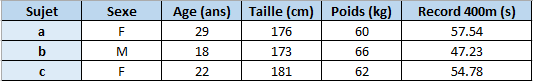
\includegraphics[scale=1]{images/tab_caracteristiques}
                    \caption{\label{fig:tab-caracteristiques}Caractéristiques des sujets}
                \end{figure}
            
            
            \subsection{Matériel}
            
                Pour réaliser l'étude le matériel suivant a été utilisé : 
                
                \begin{itemize}
                    \item un chronomètre manuel pour prendre le temps des athlètes lors la course de 400 m,
                    \item des gants en latex stériles,
                    \item des compresses stériles pour nettoyer le doigt des athlètes avant et après le prélèvement,
                    \item de l'alcool à 70°, pour nettoyer le doigt des athlètes avant et après le prélèvement,  
                    \item un stylo piqueur et des lancettes en métal, pour faire la piqûre au niveau de la pulpe du doigt et avoir un échantillon de sang à prélever,
                    \item des bandelettes de test Lactate Pro pour récupérer la goutte de sang,
                    \item un lactatomètre « Lactate Pro » de la marque ARKRAY pour mesurer la lactatémie,
                    \item un glucomètre pour mesurer la glycémie,
                    \item un oxymètre de poul de la marque Sanitas pour mesurer l'oxymétrie de pouls,
                    \item une montre Garmin Forerunner 235 pour mesurer la fréquence cardiaque.\\
                \end{itemize}
        
    
        \subsection {Déroulement des tests}
        
            L'objectif de notre travail est de comparer chez 3 athlètes la concentration sanguine de lactate (lactatémie), le taux de glucose sanguin (glycémie), la saturation pulsée en oxygène (oxymétrie de pouls) et la fréquence cardiaque avant et après une course de 400 m pour ensuite étudier les relations qui pourraient exister entre ces différents paramètres et enfin pouvoir comprendre la performance réalisée. \\
            
            Le plan expérimental se déroule sur 5 jours durant une semaine de stage où les trois athlètes sont dans les mêmes conditions : même alimentation, mêmes entraînements, mêmes heures de sommeil. \\
            
            Les tests ont eu lieu sur une piste d'athlétisme qui répond aux normes internationales de l'IAAF (Fédération Internationale d'Athlétisme). Elle se situe sur le stade municipal Romeo Neri à Rimini, en Italie.\\
            
            Les 3 sujets étaient répartis dans 3 groupes différents pour pouvoir effectuer les mesures chacun leur tour.\\
            
            Ils ont réalisé un 400 mètres à 12h30 les deux premiers jours du stage, puis ont eu un jour de repos et ont à nouveau réalisé un 400m les deux jours suivants.\\

            L'intensité du 400 mètres était maximale, c'est à dire qu'il était couru le plus rapidement possible, comme s'il était réalisé en compétition. \\
            
            Chaque course était précédée d’un échauffement d’une heure qui était le même pour les trois athlètes. L'échauffement été composé de 15 minutes de footing à une allure de 11 km/h, d'étirements, de gammes de course (talons fesses, montées de genoux, jambes tendus), de trois accélérations sur 80 mètres et enfin de trois départs en sprint sur 20 mètres.\\
            
            La saturation pulsée en oxygène a été mesurée avec l'oxymètre de pouls 2 minutes avant la course et juste après la fin de l'effort.\\
            
            La mesure de la fréquence cardiaque a été relevée sur la montre cardi-fréquencemètre 2 minutes avant la course et pendant la minute suivant l'arrêt de l'effort.\\
            
            Les échantillons de sang veineux pour la lactatémie et la glycémie ont quant à eux été prélevés  2 minutes avant la course et à partir de la 3ème minute de récupération.\\
            
            Avant le prélèvement, l'index de l'athlète était nettoyé avec une compresse et de l'alcool à 70°. La première goutte de sang qui apparaissait était aspirée par la bandelette du lactatomètre et la deuxième par celle du glucomètre.\\
            
            Le délai de prélèvement n'a jamais excédé 5 minutes.\\
         
            
            \subsection {Traitement statistique}
             
                Après avoir recueilli les données, ces dernières ont étés traitées grâce au logiciel de statistique R afin d'analyser l'existence ou non d'une relation entre lactatémie, glycémie, oxymétrie de pouls, fréquence cardiaque et la performance notamment. \\
                
                L'hypothèse posée est l'hypothèse nulle, ou H0, c'est à dire que les deux variables observées sont indépendantes.\\
                 
                Le rejet de l'hypothèse nulle implique donc l'existence d'une relation entre les deux variables observées.\\
    
                La prise de décision de rejet ou non de l’hypothèse nulle dépend de la probabilité de faire une erreur (p-valeur), c'est à dire de rejeter l'hypothèse nulle alors qu'elle est vraie. Nous appellerons la p-value p.\\
                
                La limite acceptable d'erreur a été fixée à 5\% (\si{\alpha}= 0,05).\\
                
                Nous dirons que:
                  \begin{itemize}
                      \item si la probabilité de faire une erreur (p-valeur) est inférieure à \si{\alpha} alors l'hypothèse H0 est rejetée et les variables sont dépendantes;
                      \item si la probabilité de faire une erreur (p-valeur) est supérieure à la probabilité \si{\alpha} alors l'hypothèse H0 est acceptée et les variables sont indépendantes.\\
                  \end{itemize}
              
                Pour mesurer l'intensité de la liaison entre les deux variables, le calcul du coefficient de corrélation, noté r, a été effectué. \\

                Le coefficient de corrélation est compris entre -1 et 1. Plus ce dernier est proche de -1 ou 1, plus la relation entre les deux variables est forte. On dit alors qu'elles sont fortement corrélées.\\
                
                Le coefficient est positif et la droite qui représente la corrélation est croissante si les deux variables ont tendance à augmenter ou à diminuer ensemble. Il est négatif et la droite décroissante si une variable a tendance à augmenter lorsque l'autre diminue.\\
                
                Un coefficient de corrélation nul signifie que les deux variables ne sont pas linéairement corrélées.\\ 
                 
                Pour résumé, en fonction du coefficient de corrélation, on dira que la relation entre les deux variables observées est :

                 \begin{figure}[H]
                    \centering 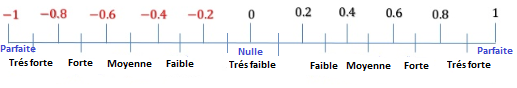
\includegraphics[scale=1]{images/coeff_corr}
                \end{figure}
            
 
              Enfin, pour être interprété, le coefficient de corrélation doit être significatif c'est à dire que la p-valeur doit être plus petite que le seuil fixé (ici 0,05).
 
 
    \section{Présentation des résultats}
    
        Toutes les données ont été stockées sous forme tabulaire dans des fichiers .csv et sont disponibles dans les Annexes (p.\pageref{annexe}).\\
        
        Les valeurs des variables biologiques qui ont étés analysées sont celles prélevées avant et après le 400 mètres, mais aussi l'écart entre ces deux mesures.\\
    
        \subsection{Fréquence cardiaque}
        \label{section:resfc}
        
        Les valeurs brutes de la fréquence cardiaque sont disponibles dans l'\autoref{annexe_fc}.\\
         
        Les graphiques ci-dessous (fig. \ref{fig:fc_perf_moy_seule}) présentent la relation entre la performance réalisée et la fréquence cardiaque avant le 400m puis après le 400m.\\ 
         
         \begin{figure}[H]
                \centering
                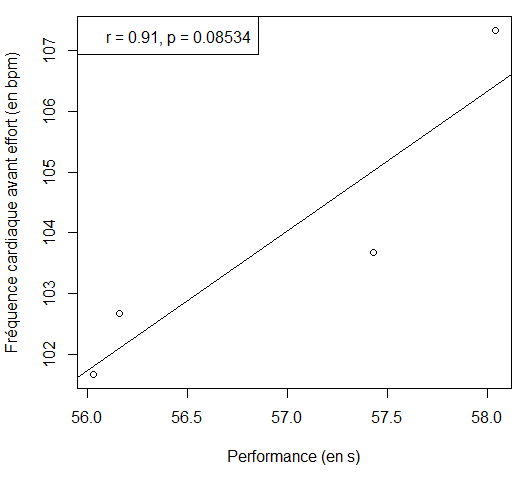
\includegraphics[scale=0.6]{images/fc_perf_av_moy_seule}
                \hfill
                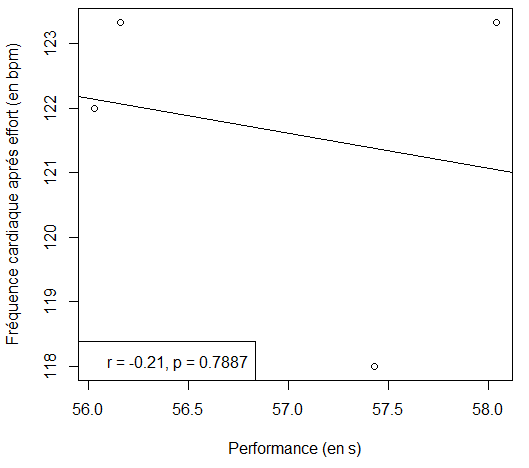
\includegraphics[scale=0.6]{images/fc_perf_ap_moy_seule}
                \caption{\label{fig:fc_perf_moy_seule}Relation entre la fréquence cardiaque avant la course (à gauche) et après (à droite) et la performance réalisée.}
            \end{figure}
            
          Les coefficients de corrélation trouvés indiquent qu'en moyenne il existe une relation très forte entre la fréquence cardiaque avant la course et le temps réalisé (r=0,91).\\
          
          Nous pouvons remarquer que la relation entre la fréquence cardiaque après la course et la performance est quant à elle très faible (r=-0,21).\\
         
 
         Enfin, les résultats présentés dans le graphique ci-dessous (fig. \ref{fig:fc_perf_ecart_moy_seule}) exposent une très forte relation (r=0,88) entre la performance réalisée et l'écart moyen de la fréquence cardiaque entre les valeurs avant un 400m et celles après .\\
         
         \begin{figure}[H]
                \centering
                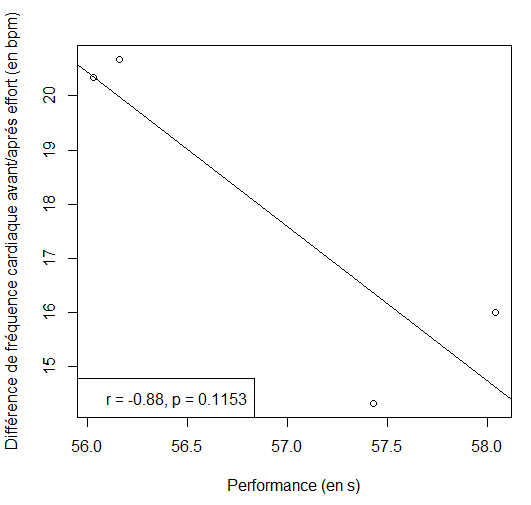
\includegraphics[scale=0.6]{images/fc_perf_ecart_moy_seule}
                \caption{\label{fig:fc_perf_ecart_moy_seule}Relation entre la performance réalisée et l'écart moyen de la fréquence cardiaque avant et après la course.}
            \end{figure}
            
            
        \subsection{Oxymétrie de pouls}
        \label{section:resOxy}
        
            Les valeurs brutes de l'oxymétrie de pouls sont disponibles dans l'\autoref{annexe_oxy}.\\
             
            Le tableau ci-dessous (fig. \ref{fig:oxy_recap}) présente les valeurs moyennes de l'oxymétrie de pouls en fonction de la performance réalisée par les trois sujets.\\
    
            \begin{figure}[H]
                \centering
                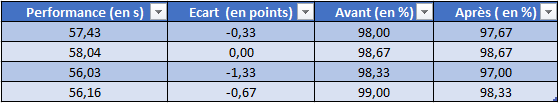
\includegraphics[scale=1]{images/oxy_recap}
                \caption{\label{fig:oxy_recap}Oxymétrie de pouls en fonction des performances réalisées sur les 4 jours de test par les 3 sujets.}
            \end{figure}
            
            Nous pouvons constater que les valeurs ne varient pratiquement pas. De ce fait nous ne pouvons pas supposer de relation particulière entre l'oxymétrie de pouls et la performance réalisée.\\
        
      
        \subsection{Glycémie}
        \label{section:resGlycemie}
        
            Les valeurs brutes de la glycémie obtenue sont présentées dans l'\autoref{annexe_gly}.\\
             
            Le graphique ci-dessous (fig. \ref{fig:gly_ecart}) décrit les écarts qui existent entre les valeurs de la glycémie avant le 400m et celles après. \\
            
            Nous pouvons remarquer que ces écarts sont toujours positifs c'est à dire que la glycémie est toujours plus élevée après le 400 mètres qu'avant.
    
            \begin{figure}[H]
                \centering
                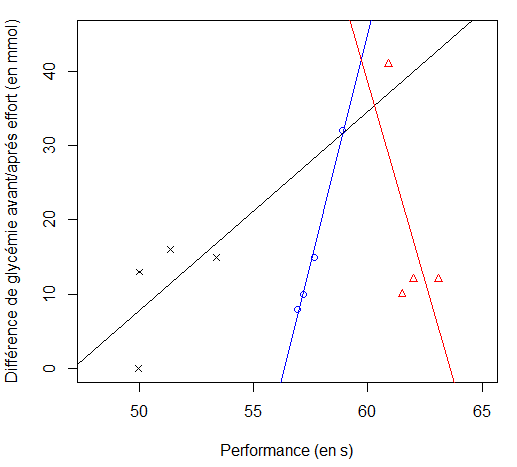
\includegraphics[scale=0.7]{images/gly_ecart}
                \caption{\label{fig:gly_ecart}Écart de glycémie entre les valeurs avant et celles après le 400m. Les symboles similaires font référence aux mêmes sujets.}
            \end{figure}
            
            
            Le graphique suivant (fig. \ref{fig:gly_perf_av}) présente la relation entre la performance réalisée et la glycémie avant le 400m.\\
            
            \begin{figure}[H]
                \centering
                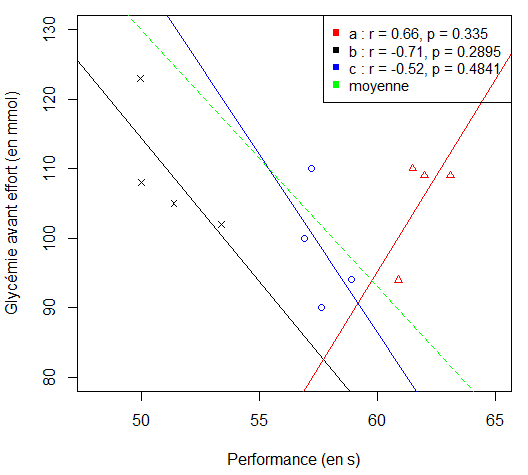
\includegraphics[scale=0.7]{images/gly_perf_av_moy}
                \caption{\label{fig:gly_perf_av}Relation entre la performance réalisée et la glycémie avant le 400m. Les symboles similaires font référence aux mêmes sujets.}
            \end{figure}
            
            Les coefficients de corrélation trouvés montrent qu'il existe bien une relation entre la performance et la glycémie avant la course pour les trois sujets (respectivement r= 0,66, r=-0,71 et r=-0,52). La moyenne indique une corrélation positive.\\
        
            Notons qu'aucun résultat intéressant n'a été trouvé concernant les valeurs de la glycémie après le 400m et la performance réalisée.\\
        
        
        \subsection{Lactatémie}
        \label{section:resLact}
        
            Les valeurs brutes de la lactatémie sont présentées dans l'\autoref{annexe_lact}.\\
            
            Les graphiques ci-dessous (fig. \ref{fig:lact_perf_av_ap}) présentent la relation entre la performance réalisée et lactatémie avant le 400m, puis après le 400m  pour chacun des sujets.\\
                   
            \begin{figure}[H]
                    \centering
                    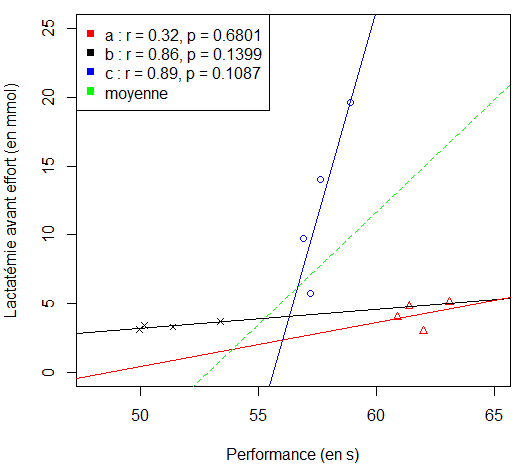
\includegraphics[scale=0.6]{images/lact_perf_av_moy}
                    \hfill
                    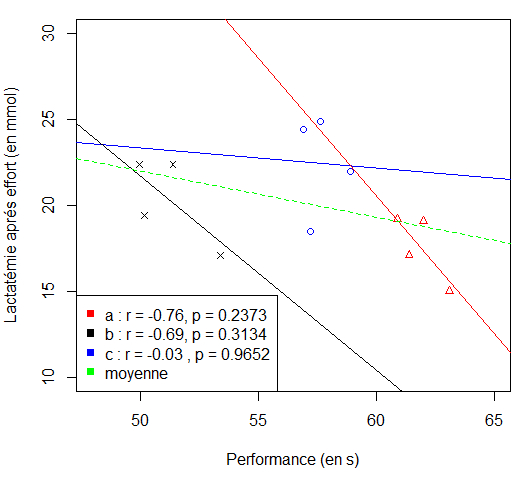
\includegraphics[scale=0.6]{images/lact_perf_ap_moy}
                    \caption{\label{fig:lact_perf_av_ap}Relation entre la performance réalisée sur une épreuve de 400m et la lactatémie avant la course (à gauche) et après (à droite). Les symboles similaires font référence aux mêmes sujets.}
            \end{figure}
            
            Au vue des coefficients de corrélation obtenus après les tests de régression linéaire, nous pouvons affirmer qu'il existe une relation entre la performance réalisée et la valeur de la lactatémie avant le 400m. La moyenne indique une très forte relation entre ces deux variables (r=0.84).\\
            
            Concernant la relation entre la performance réalisée et la valeur de la lactatémie après le 400m, la moyenne nous montre que la relation entre ces deux variables est faible (r=-0.29).\\
            
            Enfin, les résultats présentés dans le graphique ci-dessous (fig. \ref{fig:lact_perf_ecart}) montrent qu'il existe une forte relation entre la performance réalisée et l'écart de lactatémie entre les valeurs avant un 400m et celles après (respectivement r=-0,64, r=-0,71 et r=-0,997 pour les sujets a, b et c). La moyenne indique une très forte corrélation (r= -0.97) avec des résultats statistiquement significatifs (p=0.03).

                    
             \begin{figure}[H]
                    \centering
                    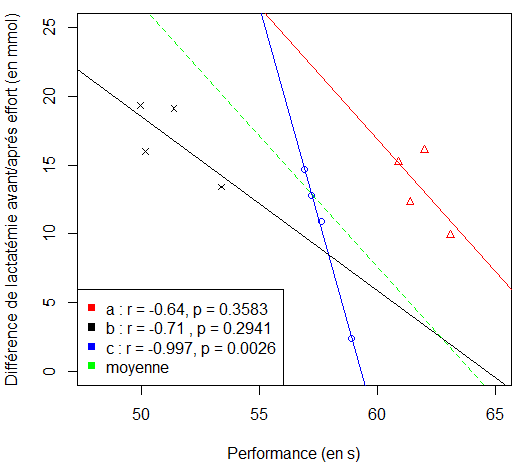
\includegraphics[scale=0.6]{images/lact_perf_ecart_moy}
                    \caption{\label{fig:lact_perf_ecart}Relation entre la différence de lactatémie avant et après le 400m et la performance réalisée. Les symboles similaires font référence aux mêmes sujets.}
            \end{figure}
        
        
    \section{Discussion}
    
        \subsection{La fréquence cardiaque et la performance réalisée}
        
        Les résultats que nous avons obtenus montrent qu'il existe une forte relation entre la performance et la valeur de la fréquence cardiaque avant un 400m. Nous remarquons qu'en moyenne, plus la fréquence cardiaque est faible avant la course, meilleur est le temps réalisé.\\
        
        De la même façon, la forte relation qui est exposée entre la différence de fréquence cardiaque avant et après la course et la performance réalisée indique que plus l'athlète est capable d'avoir une fréquence cardiaque basse avant le 400m et une fréquence cardiaque haute après, meilleure est la performance. \\
        
        En outre, les résultats montrent que la fréquence cardiaque après la course n'a pas vraiment de relation avec le temps réalisé. Cela peut être expliqué par le fait que la fréquence cardiaque dépend beaucoup des personnes. Certains ont une fréquence cardiaque qui augmente très rapidement après un exercice intense, mais ce n'est pas le cas pour d'autres.\\
        
        Je pense qu'il aurait été plus intéressant de mesurer la V02max pour connaître l'intensité de l'exercice effectué comme cela a été réalisé par A. P.CHASSAIN dans son étude \cite{chassain86}.
       

        \subsection{L'oxymétrie de pouls et la performance réalisée}
         
        Les résultats obtenus par la mesure de l'oxymétrie de pouls ne sont pas exploitables, car ils n'ont pas été fait dans les bonnes conditions. En effet, pour pouvoir observer des changements du taux d'oxygène dans le sang, il aurait fallu mesurer l'oxymétrie de pouls pendant l'effort. Cependant, cela demande du matériel que nous n'avions pas en notre possession, comme un masque de mesure d'oxygène par exemple.
         
         
        \subsection{La glycémie et la performance réalisée}
    
            La relation qui existe entre la glycémie avant la course et la performance réalisée indique qu'en moyenne, plus le taux de glucose sanguin d'un athlète avant le 400m est important, plus sa performance sera bonne par rapport à ses autres courses. Cela est cohérent : plus les muscles ont du glucose à disposition, plus ils pourront en consommer pour produire de l'énergie et finalement être plus efficace.\\
                
            Toutefois, l'augmentation de la glycémie avant une course ne peut pas être effectuée de la même façon suivant l'épreuve réalisée. Comme nous l'avons expliqué précédemment (cf. 1.2.1.\ref{ig}), les aliments n'ont pas tous le même indice glycémique et de ce fait la libération de l'énergie ne se fera pas dans les mêmes délais en fonction de l'absorption d'un aliment à IG bas, moyen ou élevé. L'ingestion d'un aliment à IG élevé moins de 30 minutes avant la course ne poserait pas de problème, voir pourrait être bénéfique pour un coureur de 400m, mais cela pourrait être risqué pour un coureur de 800m par exemple. Certes la première minute de course sera rapide du fait de la grande quantité de glucose et d'énergie disponible, mais très rapidement l'athlète se trouvera dans un état d'hypoglycémie du fait du manque de glucose qui aura été complètement utilisé. La fin de course s'avèrera donc compliquée.\\
                
            Concernant la glycémie après le 400m, la logique voudrait que celle-ci soit moins élevée qu'avant cet effort puisque pour assurer l'exercice, les muscles ont besoin d'énergie et consomment donc du glucose. Cependant, l'écart de glycémie entre la valeur d'arrivée et la valeur de départ est toujours positif ce qui indique que la glycémie est toujours plus élevée après le 400m qu'avant.\\
            
            Ces résultats étaient déjà ceux exposés par T.D. JUSTICE \cite{justice15}, mais se confirment dans la présente étude.\\
                
            Nous pouvons expliquer cela par le fait que lors d'une compétition ou d'un effort de courte durée, mais intense ou violent, l'athlète est généralement soumis au stress physique et/ou psychologique. Dans ce cas, le corps déclenche une augmentation des hormones de contre-régulation (cf. p.\pageref{glycemie}). Les hormones de stress ainsi sécrétées dans le corps provoquent la libération de sucre dans le sang et de ce fait une augmentation de la glycémie.\\
            
        
        \subsection{La lactatémie et la performance réalisée}
        
            
            Dans leur étude, J.R LACOUR et coll. \cite{lacour90} affirmaient qu'il y avait une forte relation entre la valeur de la lactatémie après un 400m et la performance réalisée (r=0.85). D'après eux, la concentration de lactate sanguin après une course était d'autant plus importante que l'athlète se rapprochait de sa meilleure performance de la saison. \\
            
            D'après mes résultats, il est vrai que la valeur de la lactatémie après le 400m est un indicateur important, mais ce n'est pas cette valeur qui explique la performance. En effet, elle ne signifie pas que plus la lactatémie est haute, plus l'athlète court vite, mais plutôt que plus la lactatémie est haute, plus l'athlète est \textbf{capable} de courir vite.  \\
            
            Comme l'a exposé F. PERONNET dans son étude \cite{peronnet13}, la concentration maximale possible de lactate est d'environ 30 mmol/l. Ainsi, si l'on remarque qu'a l'issue de chacune de ses courses un athlète n'atteint pas des valeurs de lactatémie élevées, c'est à dire que celles-ci ne dépassent jamais 20 mmol/l, cela signifie que l'athlète devra travailler sa capacité de production de lactate à l'entraînement pour augmenter ces valeurs. C'est précisément le cas du sujet A dans cette étude. De la même façon, même si un athlète présente des valeurs de lactatémie élevées (autour de 23 mmol/l), l'objectif de l'entraînement sera également d'augmenter sa capacité de production de lactate dans le but d'atteindre les valeurs maximales. \\
            
            La valeur de la lactatémie après le 400m est donc un indicateur de la capacité de production de lactate de l'athlète et par conséquent de sa capacité à courir vite, mais ce n'est pas elle qui explique la performance.\\ 
            
            J.R LACOUR et coll. ont obtenus de tels résultats, car ils se sont limités à la mesure de la lactatémie après effort et n'ont pas mesuré la concentration de lactate avant la course, ni l'écart qu'il pouvait exister entre la valeur d'arrivée et la valeur de départ de celle-ci.\\
            
            Typiquement, si nous prenons l'exemple du sujet C, la valeur de sa lactatémie après une course réalisée en 58,90s était de 22 mmol/l. Le sujet a ensuite réalisé une autre course en 57,21s et nous avons relevé une lactatémie après course de 18,5 mmol/l. Le fait que la lactatémie soit plus élevée lors de la course la plus lente confirme que ce n'est pas la forte production de lactate qui induit une meilleure performance. \\
            
            Ce phénomène s'explique ici par la valeur de la lactatémie avant le 400m. Celle ci était égale à 19,6 mmol/l lors de la première course et à 5,7 mmol/l lors de la deuxième. Il est logique que lorsqu'une course est débutée avec une lactatémie déjà élevée, cela engendre des valeurs plus élevées à l'arrivée.\\
        
            Les résultats obtenus par la présente étude ne sont donc pas en concordance avec ceux de J.R LACOUR et coll., car ils mettent en évidence le fait que ce n'est pas la valeur de la lactatémie après le 400 mètres qui est liée à la performance, mais plutôt l'écart observé entre la valeur de départ et la valeur d'arrivée de la lactatémie.\\
        
            Nous remarquons que pour un athlète, plus cet écart est important, meilleur est son temps réalisé par rapport à ses autres courses. Pour le sujet C, la corrélation entre l'écart de lactatémie avant et après le 400m et le chrono réalisé est pratiquement égale à 1 ce qui prouve une relation presque parfaite. L'écart de lactatémie serait donc un des points qui permettrait d'atteindre le meilleur niveau de performance pour un athlète.\\
           
            Il est néanmoins important de noter que cette observation ne peut pas être généralisée. Nous ne pouvons pas affirmer que plus la différence entre la lactatémie avant et après effort est grande, plus la performance réalisée est bonne. En effet, certaines variables de la composition corporelle comme le genre, le poids, le poids idéal, la masse graisseuse, etc ou même des éléments extérieurs comme le vent peuvent influer sur la production de lactate dans le sang. Par exemple, nous pouvons constater que le sujet C avait un écart de 2,4 mmol/l lorsqu'il a couru en 58.90s alors que le sujet A avait un écart de 16,1 mmol/l pour courir 3 secondes plus lentement (en 61.99s). Ceci signifie simplement que si le sujet C avait un écart plus grand, il courait plus vite. Cela est donc relatif à chaque athlète.\\
            
            Lors de l'analyse des données des deux premiers jours de l'étude, nous avons constaté des valeurs anormalement haute de la lactatémie avant le 400m pour le sujet C. En effet, celles-ci étaient égales à 19,6 mmol/l et à 14 mmol/l tandis que les sujets A et B avaient des valeurs proches de 3,5 mmol/l. L'écart entre les valeurs avant et après l'effort était donc faible et respectivement de 2,4 mmol/l et de 10,9 mmol/l.\\
            
            Nous avons alors décidé de modifier le protocole d'échauffement du sujet C pour analyser si ce dernier favorisait l'augmentation de la production de lactate dans le sang. Le sujet C devait alors réaliser le même échauffement que précédemment, mais l'avoir terminé 15 minutes avant le début de sa course et rester assis jusqu'à 1 minute avant sa course.\\
            
            Les résultats ont été sans appel. La lactatémie des deux jours suivant était égale à 5,7 mmol/l puis à 9,7 mmol/l ce qui a permis d'obtenir des écarts plus importants entre la valeur d'arrivée et la valeur de départ (respectivement de 12,8 mmol/l et de 14,7 mmol/l). Les performances se sont également largement améliorées passant de 58.90s et 57.65s les deux premiers jours, à 57.21s et 56.91s après la modification de l'échauffement.\\
            
            L'analyse de la lactatémie des sujets a donc été la mesure qui a permis de faire la découverte majeure de cette étude. Nous pouvons aujourd'hui avancer que l'une des clés de la performance au 400m est d'être capable de produire de grandes quantités de lactate tout en ayant des valeurs de lactatémie très basse avant la course. 

        
    \section{Menaces à la validité de l'étude}
        
        Il faut reconnaître que notre étude présente des limites. Une des menaces principale à la validité de cette étude est que l'échantillon observé (n=3) est trop petit. Cela pose problème, car la p-valeur est généralement supérieure au seuil fixé (\si{\alpha}= 0,05) ce qui montre que les résultats ne sont statistiquement pas significatifs. \\
        
        En outre, les mesures de la saturation pulsée en oxygène et de la fréquence cardiaque n'ont pas été effectuées de sorte à trouver des résultats intéressants. En effet, les mesures auraient du être prise pendant la course et non avant ou après. De cette façon nous aurions pu déceler des variations significatives et en tirer les conclusions qui s'imposent.\\
        

            
    \section{Perspectives}
        
        De multiples perspectives sont prévues pour cette étude. Tout d'abord l'étude va être poursuivie, mais avec un échantillon plus grand. L'objectif est d'avoir un échantillon composé de 10 à 15 sujets.\\
     
        Ensuite, la mesure de la fréquence cardiaque sera mesurée pendant l'effort grâce à un cardio-fréquencemètre qui enregistre les pulsations durant toute la durée de la course.\\
        
        Nous mesurerons également la VO2max, car cette valeur est un bon indicateur de l'intensité de l'effort produit. \\
        
        Par ailleurs, l'idéal serait d'obtenir un masque pour pouvoir mesurer le taux d'oxygène dans le sang pendant l'effort. \\
        
        Après avoir récolté ces données, cela pourrait être intéressant de mettre en relation la fréquence cardiaque recueillie pendant l'effort et la performance réalisée pour connaître les valeurs à partir desquelles la performance se détériore. De la même façon nous pourrons observer la VO2MAx et le taux d'oxygène dans le sang pour savoir à partir de quel intensité la quantité d'oxygène commence à diminuer. Ensuite, la lactatémie pourrait être mise en relation avec la SpO2 pour connaître le taux d'oxygène à partir duquel la production de lactate augmente significativement. \\
        
        Enfin, une suite de cette étude pourrait être d'intégrer des protocoles de méditation, d'hypnose ou de sophrologie dans le cadre de la préparation physique et mentale des athlètes afin évaluer les différences s'il y en a. Ces nouvelles démarches sont réputées pour aider l'athlète à se concentrer, à réduire le stress, mais aussi à mieux gérer la douleur. L'application de ces méthodes pourrait également avoir un effet sur les aspects physiologiques étudiés précédemment comme par exemple abaisser la fréquence cardiaque.\\
        
        L'objectif serait donc de voir à quel point l'esprit peut aider le corps dans la performance.
    
    

%%% Local Variables: 
%%% mode: latex
%%% TeX-master: "rapport"
%%% End: 
